\chapter{Contexto del proyecto}
En este capítulo se tratarán tanto los antecedentes como el estado del arte. Primeramente se expondrán los diferentes tipos de software de gestión bibliotecaria, así como su evolución. Tras ello, se explicarán brevemente las soluciones software de gestión de bibliotecas, y se describirán tanto sus ventajas como sus inconvenientes. Una vez explicadas las particularidades de cada sistema software en el estado del arte, se hará una breve comparativa de estas tecnologías con Liber. Para finalizar el capítulo, se expondrán las tecnologías utilizadas; tanto sus características como la motivación de usarlas.

\section{Antecedentes: evolución histórica de los sistemas de gestión bibliotecaria}

La gestión automatizada de bibliotecas no es un fenómeno reciente, es el resultado de una evolución tecnológica y conceptual que comienza hace más de medio siglo. Comprender su trayectoria es fundamental para situar el presente proyecto en su contexto y valorar las decisiones de diseño adoptadas durante el desarrollo.

Los orígenes de la automatización bibliotecaria mediante computación se remontan a la década de 1960, con iniciativas pioneras como el desarrollo del protocolo MARC (\textit{Machine-Readable Cataloging}) por parte de la Biblioteca del Congreso de Estados Unidos. Este estándar, que permitía el intercambio de registros bibliográficos en formato legible por máquina, estableció las bases para la creación de los primeros catálogos automatizados y marcó un hito en la estandarización de los datos bibliográficos mundialmente. La adopción de MARC facilitó la colaboración entre instituciones y creación de redes bibliotecarias, transformando profundamente los procesos de catalogación y descripción de fondos.

Entre las décadas de 1970 y 1980, los sistemas de gestión bibliotecaria experimentaron un desarrollo significativo con la aparición de los primeros ILS (\textit{Integrated Library Systems}), o SIGB (Sistemas Integrados de Gestión Bibliotecaria), en español. Estas plataformas, inicialmente concebidas para entornos \textit{mainframe}, integraban funcionalidades básicas tales como catálogos en línea, control de préstamos y adquisiciones. No obstante, se trataba de sistemas propietarios, con un coste elevado y una complejidad técnica que limitaba su rango de implantación a grandes bibliotecas universitarias y nacionales. El estudio \textit{Library Management Systems Study} \parencite{jisc2008} ofrece una panorámica detallada de este periodo, identificando los principales sistemas comerciales y sus capacidades, así como las limitaciones derivadas de su arquitectura monolítica y su escasa flexibilidad. Los sistemas integrados de gestión bibliotecaria, al igual que los recursos computacionales, era algo que solamente cierto tipo de organizaciones podía permitirse implementar durante estas décadas en las que la computación aún era algo complejo de comprender y costoso de implementar.

La consolidación del mercado de sistemas de gestión bibliotecaria en las décadas de 1990 y 2000 vino acompañada de una intensa actividad de fusiones y adquisiciones empresariales. Breeding \parencite{breeding_history} documenta gráficamente este proceso, mostrando cómo numerosos proveedores independientes fueron absorbidos por grandes conglomerados, reduciendo la diversidad del mercado y consolidando un puñado de soluciones dominantes. Este suceso, aunque permitió la integración de funcionalidades y la creación de plataformas más completas, también generó una fuerte dependencia de unos pocos proveedores y dificultó la aparición de alternativas más flexibles o adaptadas a contextos específicos; a cambio de tener unos estándares centralizados, había pocas alternativas.

A finales de la primera década del siglo XXI, el panorama de los sistemas de gestión bibliotecaria comenzó a diversificarse con la aparición de soluciones de código abierto, siendo Koha (2000) y Evergreen (2006) los exponentes más destacados. La creación de este tipo de plataformas de catalogación de código abierto surge como respuesta a la necesidad de establecer ciertos estándares de comunicación y almacenamiento de información, dado que previamente solo había complejos sistemas originados en organizaciones de gran extensión. Durante estos años, estos sistemas de catalogación se comienzan a poner al servicio de clientes más de a pie, a usuarios menos experimentados, usando tecnologías de este tipo. Estas plataformas ofrecían una alternativa a los sistemas propietarios, con modelos de desarrollo colaborativo que permitían una mayor personalización y un coste de adquisición reducido. Sin embargo, la complejidad de su implantación y mantenimiento seguía siendo un obstáculo para bibliotecas de menor tamaño. Paralelamente, la web 2.0 y el desarrollo de tecnologías como los OPACs de nueva generación transformaron las expectativas de los usuarios, que demandaban interfaces más intuitivas y funcionalidades sociales.

Asimismo, la evolución de las publicaciones hacia formatos electrónicos trajo consigo la necesidad de una gestión distinta de los recursos. Surgen así las Plataformas de Servicios Bibliotecarios (PSB), también denominadas SIGB de nueva generación. Como señala Sandra Cano \parencite{cano2021psb} en su trabajo fin de grado, \textit{``las PSB nacen de la necesidad de unificar los tradicionales flujos de trabajos de las bibliotecas con las nuevas necesidades tecnológicas de los documentos electrónicos''}. La principal razón de ser de las PSB es gestionar de manera integrada tanto materiales impresos como electrónicos, consolidando en un único sistema funciones que antes requerían de múltiples productos especializados.

Marshall Breeding estimó que para 2020 las bibliotecas académicas o de investigación usarían PSB y para 2026 serían todas las bibliotecas \parencite{breeding_history}. La principal razón por la que se pueda retrasar el acercamiento de las plataformas en las bibliotecas es debido al coste económico que supone implementar un nuevo sistema, sustituyendo a uno que ya funciona a pesar de las posibles limitaciones que tenga, y más cuando es la novedad en el mercado de los softwares de bibliotecas.

Las PSB se caracterizan por \parencite{cano2021psb}:
\begin{itemize}
	\item Relacionar los módulos entre sí (por ejemplo, asignar un usuario en concreto para un préstamo, relacionando los módulos de gestión de usuarios con el de préstamos).
	\item Utilizar una única base de datos para gestionar todas las funciones.
	\item Automatizar los procesos.
\end{itemize}

Entre las principales PSB del mercado destacan Alma (de Ex Libris, propiedad de ProQuest), Sierra (de Innovative Interfaces), y WorldShare Management Services (de OCLC). A diferencia de los SIGB tradicionales, que se adquirían mediante compra de licencia, las PSB se ofrecen bajo modelo de suscripción o de software como servicio (SaaS, Software as a Service) con precios que varían según el tamaño de almacenamiento y las funcionalidades contratadas. Además, su arquitectura \textit{multi-tenant} y basada en la nube permite a las bibliotecas acceder al sistema desde cualquier dispositivo sin necesidad de instalación local, con actualizaciones globales aplicadas por el proveedor, y con APIs expuestas que facilitan la interoperabilidad con otros sistemas.

En este contexto, el proyecto \textit{HeLibTech} \parencite{helibtech} surge como un recurso colaborativo para la comunidad de educación superior en el Reino Unido, manteniendo actualizada la información sobre el ecosistema tecnológico bibliotecario. Su enfoque comunitario y su vocación de servicio público reflejan una tendencia creciente hacia la apertura y el intercambio de conocimiento en el ámbito de la tecnología bibliotecaria, una filosofía que el presente trabajo de fin de grado comparte y promueve.

La evolución histórica evidencia que, a pesar de los avances, persisten desafíos importantes. Muchos de los sistemas actuales, tanto comerciales como de código abierto, mantienen una complejidad inherente que los hace difíciles de desplegar y mantener por personal sin una formación técnica especializada. Asimismo, la tendencia hacia soluciones monolíticas o excesivamente modulares no siempre se traduce en una experiencia de usuario satisfactoria o en una gestión eficiente para bibliotecas de dimensiones reducidas. Es en este punto donde se enmarca la propuesta del presente trabajo: el desarrollo de un sistema de gestión de bibliotecas basado en Docker que, inspirándose en las lecciones del pasado y en las tecnologías más actuales, ofrezca una alternativa sencilla, liviana y fácilmente comprensible para bibliotecas medianas y pequeñas, con un fuerte énfasis en la accesibilidad y la apertura.

\section{Estado del arte}
Recogiendo lo expuesto en los antecedentes, se puede entrever el panorama actual de las soluciones software para bibliotecas.

Hoy en día se pueden identificar dos corrientes claras; los SIGB tradicionales y las Plataformas de Servicios Bibliotecarios (PSB) más modernas. La información muestra que, pese a que los SIGB dominen en número de instalaciones, el futuro está marcado por la inteligencia artificial y la nube, herramientas características de las PSB.

Es por esto por lo que podemos decir que nos encontramos en un punto de inflexión en lo que a soluciones software para bibliotecas se refiere. Observamos un mercado maduro y marcado tradicionalmente por grandes corporaciones o agrupaciones colaborativas que día a día está siendo redefinido por las nuevas plataformas \parencite{americanlibraries2026}. Al igual que ocurre en otros muchos ámbitos relacionados con las soluciones software, los sistemas bajo licencia están dando paso a modelos bajo suscripción. Más específicamente en el ámbito de estos sistemas de gestión, se podría decir que se está pasando de una forma de gestionar la biblioteca mediante diferentes tecnologías o \textit{suites} por licencia, a un modelo más unificado, hacia software más uniformizado o monolítico que cubre todas las funciones necesarias a través de una única suscripción.

Todas estas nuevas tecnologías permiten optimizar el funcionamiento de las bibliotecas que las integran a través de nuevas funcionalidades, como el uso de la inteligencia artificial o una instalación más sencilla a través de licencia. Al tratarse normalmente de servicios SaaS, se hace más fácil el uso e instalación de las PSB frente a los tradicionales SIGB.

Sin embargo, estas nuevas soluciones también presentan severas barreras de entrada, sobre todo para bibliotecas con poco personal técnico o medios económicos limitados \parencite{americanlibraries2026}. Este tipo de instituciones no pueden permitirse contratar administradores de sistemas dedicados a comprender el software, ni asumir el coste de una PSB. Es precisamente en este punto donde se enmarca la propuesta del presente trabajo.

Ahora que tenemos plataformas en la nube para gestionar la mayoría de bibliotecas, parece ser que estamos cerca de una coyuntura en la que la mayoría de bibliotecas tendrán un sistema de gestión moderno, integrado con inteligencia artificial, y que ofrezca nuevas funcionalidades tanto para usuarios como para el personal de la propia biblioteca. Nada más lejos de la realidad; en este sector, al igual que en la mayoría, nos podemos encontrar con una gran variedad de tipos de bibliotecas. No todas las bibliotecas pueden tener las mismas necesidades, sobre todo cuando entran en juego factores como a qué está orientada su funcionalidad, a qué clase de público quiere llegar, o el tamaño sin ir más lejos.
En este contexto cuasi trascendental, aparecen una serie de herramientas recientes que parecen estar marcando el futuro próximo de estos sistemas bibliotecarios, dado que son los PSB que más apuestan por la innovación.

\subsection{Alma}
\begin{figure}[htb]
	\centering
	
\includegraphics[scale=0.5]{imagenes/exlibris.jpg}
	\caption{Logo de Alma}
	\label{fig:alma}
\end{figure}
Alma es una plataforma de servicios bibliotecarios basada en la nube desarrollada por Ex Libris \parencite{exlibris_alma_platform}, adquirida primero por ProQuest, y más tarde por Clarivate en los últimos años, y actualmente es la plataforma principal utilizada por bibliotecas académicas y nacionales, implementada en más de 2700 instituciones en todo el mundo. Alma integra las funciones de los sistemas tradicionales de gestión bibliotecaria (SIGB) con la gestión de recursos electrónicos (ERM), adoptando un modelo de Software como Servicio (SaaS) y arquitectura multi-inquilino, donde la infraestructura del servidor, el mantenimiento de la base de datos y las actualizaciones de software son gestionados por Ex Libris.

La hoja de ruta que Alma \parencite{exlibris_alma_roadmap2026} pretende seguir en 2026 muestra que el enfoque de Alma hoy día mira hacia la IA, introduciendo asistentes inteligentes de metadatos para catalogación, adquisiciones y análisis.

Por una parte, Alma tiene una funcionalidad completa, cubriendo la gestión unificada de recursos físicos, electrónicos y digitales; su arquitectura SaaS reduce la carga de mantenimiento local; la IA mejora la eficiencia de catalogación y análisis, además de ofrecer soporte de red a nivel de consorcio para bibliotecas, permitiendo compartir la información entre las mismas.

Sin embargo presenta ciertas barreras de entrada: precio elevado, modelo de suscripción, funcionalidad compleja, con una curva de aprendizaje pronunciada. Depende de proveedores comerciales, con poca flexibilidad de personalización. Para bibliotecas con recursos técnicos y presupuestarios limitados, estas características componen un obstáculo.

\subsection{WorldShare Management Services}
\begin{figure}[htb]
	\centering
	
\includegraphics{imagenes/WMS.png}
	\caption{Logo de WorldShare Management Services}
\end{figure}

WorldShare Management Services (WMS por sus siglas) es la plataforma de servicios bibliotecarios en la nube de OCLC, cuya ventaja central radica en estar construida sobre WorldCat, la red global de datos bibliotecarios más grande del mundo. En los últimos 12 meses, 48 nuevas bibliotecas se han unido a la comunidad WMS \parencite{oclc_48nuevas2026}, incluyendo instituciones como Old Dominion University y la universidad de Medellín \parencite{oclc_odu2026}. WMS soporta las funciones principales de adquisiciones, circulación, catalogación, descubrimiento, préstamo interbibliotecario y gestión de licencias.

Es una herramienta muy útil ya que tiene integración con WorldCat, permitiendo el acceso a datos bibliográficos de cientos de millones de registros, la infraestructura compartida reduce el trabajo repetitivo, además de que está desarrollada por una organización sin ánimo de lucro, con precios relativamente razonables \parencite{oclc_wms_platform}.
Por otra parte, es cierto que es un ecosistema complejo pensado para bibliotecas que colaboran internacionalmente tales como las universidades mencionadas.

Queda claro que las PSB presentan soluciones muy prácticas para los casos de uso de las bibliotecas de hoy en día, brindando una alternativa a los clásicos SIGB a la vez que ofreciendo propiedades muy competitivas. Sin embargo, y recuperando lo mencionado previamente, este proyecto se encuentra en el nicho de las bibliotecas de fondo reducido, en el cual las bibliotecas no demandan una red de interconexión para compartir catálogos, ni se hacen necesarios asistentes de inteligencia artificial. A continuación se exponen ciertas soluciones existentes dentro de este mismo nicho; software de asistencia a la gestión de las bibliotecas más pequeñas o locales, con funcionalidades más sencillas o tradicionales, pero que por otra parte tienen un uso bastante extendido.

\subsection{Koha}
\begin{figure}[htb]
	\centering
	
\includegraphics[scale=0.5]{imagenes/koha.png}
	\caption{Logo de Koha}
	\label{fig:koha}
\end{figure}

Koha es el primer SIGB de código abierto del mundo. Se empezó a desarrollar en 1999 en Nueva Zelanda por el consorcio Horowhenua Library Trust. «Koha» proviene del maorí y significa «regalo» o «dar algo a la comunidad», reflejando la filosofía colaborativa que ha marcado el proyecto desde sus inicios. Está desarrollado y distribuido bajo la licencia GNU General Public License (GPL), por lo que garantiza a las bibliotecas la libertad de usar, modificar y distribuir el software sin restricciones \parencite{koha_zenodo2025}.

El \textit{stack} tecnológico de la herramienta está compuesto por Linux, Apache, MySQL/ MariaDB y Perl. Al igual que Liber, es una herramienta basada en web, tanto para el personal bibliotecario como para los usuarios finales, contribuyendo a que el sistema sea ligero, fácil de usar, desplegar y gestionar \parencite{koha_librarytechnology_ruskin2026}. Soporta una gran variedad de estándares, entre ellos MARC21 y UNIMARC, lo que facilita la compatibilidad con otros sistemas \parencite{koha_kohasupport2025}.

La modularidad es identitaria de Koha. El sistema incluye módulos integrados para catalogación, circulación, adquisiciones, gestión de publicaciones seriadas, OPAC, informes y gestión de usuarios. Un aspecto destacable es que todos los módulos esenciales vienen incluidos en la instalación básica sin coste adicional, lo que supone una ventaja significativa frente a los sistemas propietarios que suelen cobrar por módulos o funcionalidades específicas \parencite{koha_zenodo2025}.

Entre las principales ventajas de Koha encontramos la ausencia de costes de licencia, libertad para modificar el software según las necesidades de cada biblioteca, la ausencia de dependencia de un proveedor único y el respaldo de una comunidad global muy activa, en resumidas cuentas todas las ventajas que puede tener un software de licencia GPL bien mantenido. Su adopción es notable: según datos de 2026, Koha cuenta con más de 18.000 instalaciones en todo el mundo \parencite{koha_librarytechnology_ruskin2026}, y se utiliza en bibliotecas de todo tipo, desde pequeñas bibliotecas escolares hasta grandes consorcios universitarios y redes de bibliotecas públicas.

No obstante, Koha presenta limitaciones a considerar. Su instalación y mantenimiento requieren conocimientos técnicos en Linux, Apache y MySQL, así como acceso total al servidor \parencite{koha_zenodo2025, koha_sourceforge2026}. Aunque existen servicios de \textit{hosting} gestionado que reducen esta barrera, el despliegue autogestionado sigue siendo complejo para bibliotecas sin personal técnico especializado.

Koha es una solución madura, flexible y sostenible para bibliotecas que buscan un sistema completo sin costes de licencia, pero su adopción demanda cierta complejidad técnica. Para el nicho de bibliotecas que aborda este proyecto, Koha se sitúa en un punto intermedio: ofrece más funcionalidades de las necesarias para una biblioteca pequeña y exige un nivel de infraestructura y conocimientos técnicos que pueden resultar desproporcionados.

\subsection{OpenBiblio}
\begin{figure}[htb]
	\centering
	
\includegraphics{imagenes/openbiblio.png}
	\caption{Logo de OpenBiblio}
	\label{fig:openbiblio}
\end{figure}

OpenBiblio es un SIGB de código abierto, desarrollado en PHP y MySQL, y distribuido bajo la licencia GNU General Public License (GPL). Su objetivo principal es cubrir las necesidades de automatización de bibliotecas pequeñas, ofreciendo una herramienta sencilla que no requiere una infraestructura técnica compleja \parencite{bwalya2017openbiblio, openbiblio_docs}.

A diferencia de Koha, cuyo despliegue exige conocimientos avanzados de Linux, Apache y Perl, OpenBiblio está diseñado para ser fácil de instalar y configurar. La documentación oficial describe su instalación tanto en Windows como en Linux mediante entornos como EasyPHP o servidores compartidos, con requisitos mínimos.

El sistema se organiza en cuatro módulos que representan las funciones esenciales de una biblioteca pequeña: Catalogación, Circulación, OPAC y Gestión de Usuarios. Permite la importación de registros MARC y CSV, así como la catalogación manual \parencite{vimalkumar2005}.

La ventaja más importante de OpenBiblio radica en su simplicidad. No requiere personal técnico especializado para su puesta en marcha y mantenimiento, y su curva de aprendizaje es notablemente inferior a la de otras soluciones de código abierto. Sin embargo, la sencillez también implica limitaciones: carece de módulos avanzados como adquisiciones, control de publicaciones seriadas o gestión de recursos electrónicos, y su OPAC no es tan avanzado para búsquedas en comparación con sistemas más completos \parencite{vimalkumar2005}.

Otra desventaja señalada en la literatura es la escasez de documentación actualizada en Internet, lo que puede dificultar la resolución de problemas para usuarios \parencite{bwalya2017openbiblio}. No obstante, el proyecto mantiene una comunidad activa y dispone de documentación oficial accesible en GitHub, que cubre desde la instalación hasta la administración del sistema \parencite{openbiblio_docs}.

En el contexto de este proyecto, OpenBiblio representa el extremo opuesto del espectro: es la solución más ligera y accesible entre opciones de código abierto, pero su arquitectura (PHP/MySQL) y su limitado conjunto de funcionalidades no ofrecen la flexibilidad ni la modernidad que se buscan en una aplicación web contemporánea. Esto refuerza la necesidad de una alternativa que combine la simplicidad de OpenBiblio con las capacidades de un framework moderno como Django.

\subsection{Tabla comparativa}
Con el objeto de exponer más visualmente las principales diferencias entre las soluciones software expuestas, se ha elaborado una tabla que nombra las características de cada sistema en diferentes aspectos:
\newpage
\thispagestyle{empty}
\begin{table}[H]
	\vspace{-1cm}
	\centering
	\caption{Cuadro comparativo de las soluciones de gestión bibliotecaria analizadas.}
	\label{tab:comparativa_soluciones}
	\small
	\begin{tabularx}{\textwidth}{p{2.5cm} X X X X X}
		\toprule
		\textbf{Característica} & \textbf{Alma} & \textbf{WMS} & \textbf{Koha} & \textbf{OpenBiblio} & \textbf{Liber} \\
		\midrule
		
		\textbf{Tipo} & PSB comercial & PSB comercial & SIGB open source & SIGB open source & SIGB open source \\
		\addlinespace
		
		\textbf{Desarrollador} & Ex Libris (Clarivate) & OCLC & Comunidad Koha & Comunidad OpenBiblio & Proyecto propio \\
		\addlinespace
		
		\textbf{Licencia} & Propietaria & Propietaria & GPL & GPL & GPL \\
		\addlinespace
		
		\textbf{Modelo de despliegue} & SaaS & SaaS & Autoalojado o hosting gestionado & Autoalojado & Contenerizado (Docker) \\
		\addlinespace
		
		\textbf{Stack} & Propietario & Propietario & Linux, Apache, MySQL/MariaDB, Perl & PHP, MySQL & Python, Django, PostgreSQL \\
		\addlinespace
		
		\textbf{Requisitos técnicos} & Bajos & Bajos & Medios-altos & Bajos-medios & Bajos \\
		\addlinespace
		
		\textbf{Costes} & Suscripción elevada & Suscripción moderada & Sin licencia (costes de hosting) & Sin licencia (costes de hosting) & Sin licencia (costes de hosting)\\
		\addlinespace
		
		\textbf{Módulos principales} & Catalogación, circulación, adquisiciones, ERM, analíticas, descubrimiento & Adquisiciones, circulación, catalogación, descubrimiento, ILL, licencias & Catalogación, circulación, adquisiciones, seriadas, OPAC, informes & Catalogación, circulación, OPAC, usuarios & Catalogación, circulación, usuarios, OPAC \\
		\addlinespace
		
		\textbf{Gestión de recursos electrónicos} & Sí, nativa y avanzada & Sí, integrada & Parcial & No & No \\
		\addlinespace
		
		\textbf{Alcance} & Grandes consorcios y bibliotecas nacionales & Redes internacionales de bibliotecas & Desde pequeñas bibliotecas hasta grandes consorcios & Bibliotecas pequeñas & Bibliotecas medianas-pequeñas \\
		\addlinespace
		
		\textbf{Público objetivo} & Bibliotecas académicas y nacionales & Bibliotecas académicas y redes internacionales & Bibliotecas de cualquier tamaño & Bibliotecas pequeñas y rurales & Bibliotecas medianas-pequeñas \\
		\addlinespace
		
		\bottomrule
	\end{tabularx}
\end{table}

\newpage

\section{Tecnologías utilizadas}

Liber ha sido desarrollada utilizando Django como framework principal, junto con una serie de herramientas de apoyo para facilitar el desarrollo, las pruebas, el despliegue y la gestión del código.

A continuación, se enumeran las principales características de las tecnologías empleadas, divididas en backend, base de datos, herramientas de desarrollo y documentación.

\subsection{Backend}

\subsubsection{Django}
\begin{figure}[htb]
	\centering
	
\includegraphics[width=3cm]{imagenes/django.png}
	\caption{Logo de Django}
	\label{fig:django}
\end{figure}

Django es un \textit{framework} de desarrollo web de alto nivel escrito en Python. Sigue el patrón de diseño \textit{Modelo-Vista-Template} (MVT), muy similar al Modelo-Vista-Controlador, y promueve el principio DRY (\textit{Don't Repeat Yourself}), lo que facilita la creación de aplicaciones web robustas y mantenibles.

Características principales del \textit{framework}:
\begin{itemize}
	\item Framework completo con ORM integrado, sistema de autenticación, panel de administración y gestión de formularios.
	\item Arquitectura MVT que separa la lógica de negocio, la presentación y el acceso a datos.
	\item ORM que permite interactuar con la base de datos mediante código Python, sin escribir SQL manualmente.
	\item Sistema de migraciones que versiona los cambios en el esquema de la base de datos.
	\item Panel de administración autogenerado que facilita la gestión de los modelos de datos.
	\item Compatibilidad con múltiples bases de datos (PostgreSQL, MySQL, SQLite, etc.).
	\item Enrutamiento de URLs limpio y flexible mediante expresiones regulares o convertidores de ruta.
\end{itemize}

\subsection{Base de datos}

\subsubsection{PostgreSQL}
\begin{figure}[htb]
	\centering
	
\includegraphics[width=3cm]{imagenes/postgresql.png}
	\caption{Logo de PostgreSQL}
	\label{fig:postgresql}
\end{figure}

PostgreSQL es un sistema de gestión de bases de datos relacional de código abierto, conocido por su robustez, integridad y cumplimiento de estándares SQL.

Características principales:
\begin{itemize}
	\item Soporte completo de transacciones ACID.
	\item Integridad referencial mediante claves primarias, foráneas y restricciones.
	\item Soporte para tipos de datos avanzados (JSON, arrays, rangos, etc.).
	\item Escalabilidad y alto rendimiento en entornos de producción.
	\item Integración nativa con Django a través de su ORM.
\end{itemize}

\subsection{Herramientas de desarrollo}

\subsubsection{Visual Studio Code}
\begin{figure}[htb]
	\centering
	
\includegraphics[width=3cm]{imagenes/vscode.png}
	\caption{Logo de Visual Studio Code}
	\label{fig:vscode}
\end{figure}

Visual Studio Code es un editor de código fuente ligero pero potente, desarrollado por Microsoft, que se ha convertido en uno de los editores más utilizados en el desarrollo de software.

Características principales:
\begin{itemize}
	\item Soporte nativo para múltiples lenguajes de programación, incluido Python.
	\item Extensible mediante extensiones (Python, Django, Docker, Git, etc.).
	\item Terminal integrada que permite ejecutar comandos sin salir del editor.
	\item Depurador integrado para Python y otros lenguajes.
	\item Integración con Git y GitHub para control de versiones.
\end{itemize}

\subsubsection{Docker}
\begin{figure}[htb]
	\centering
	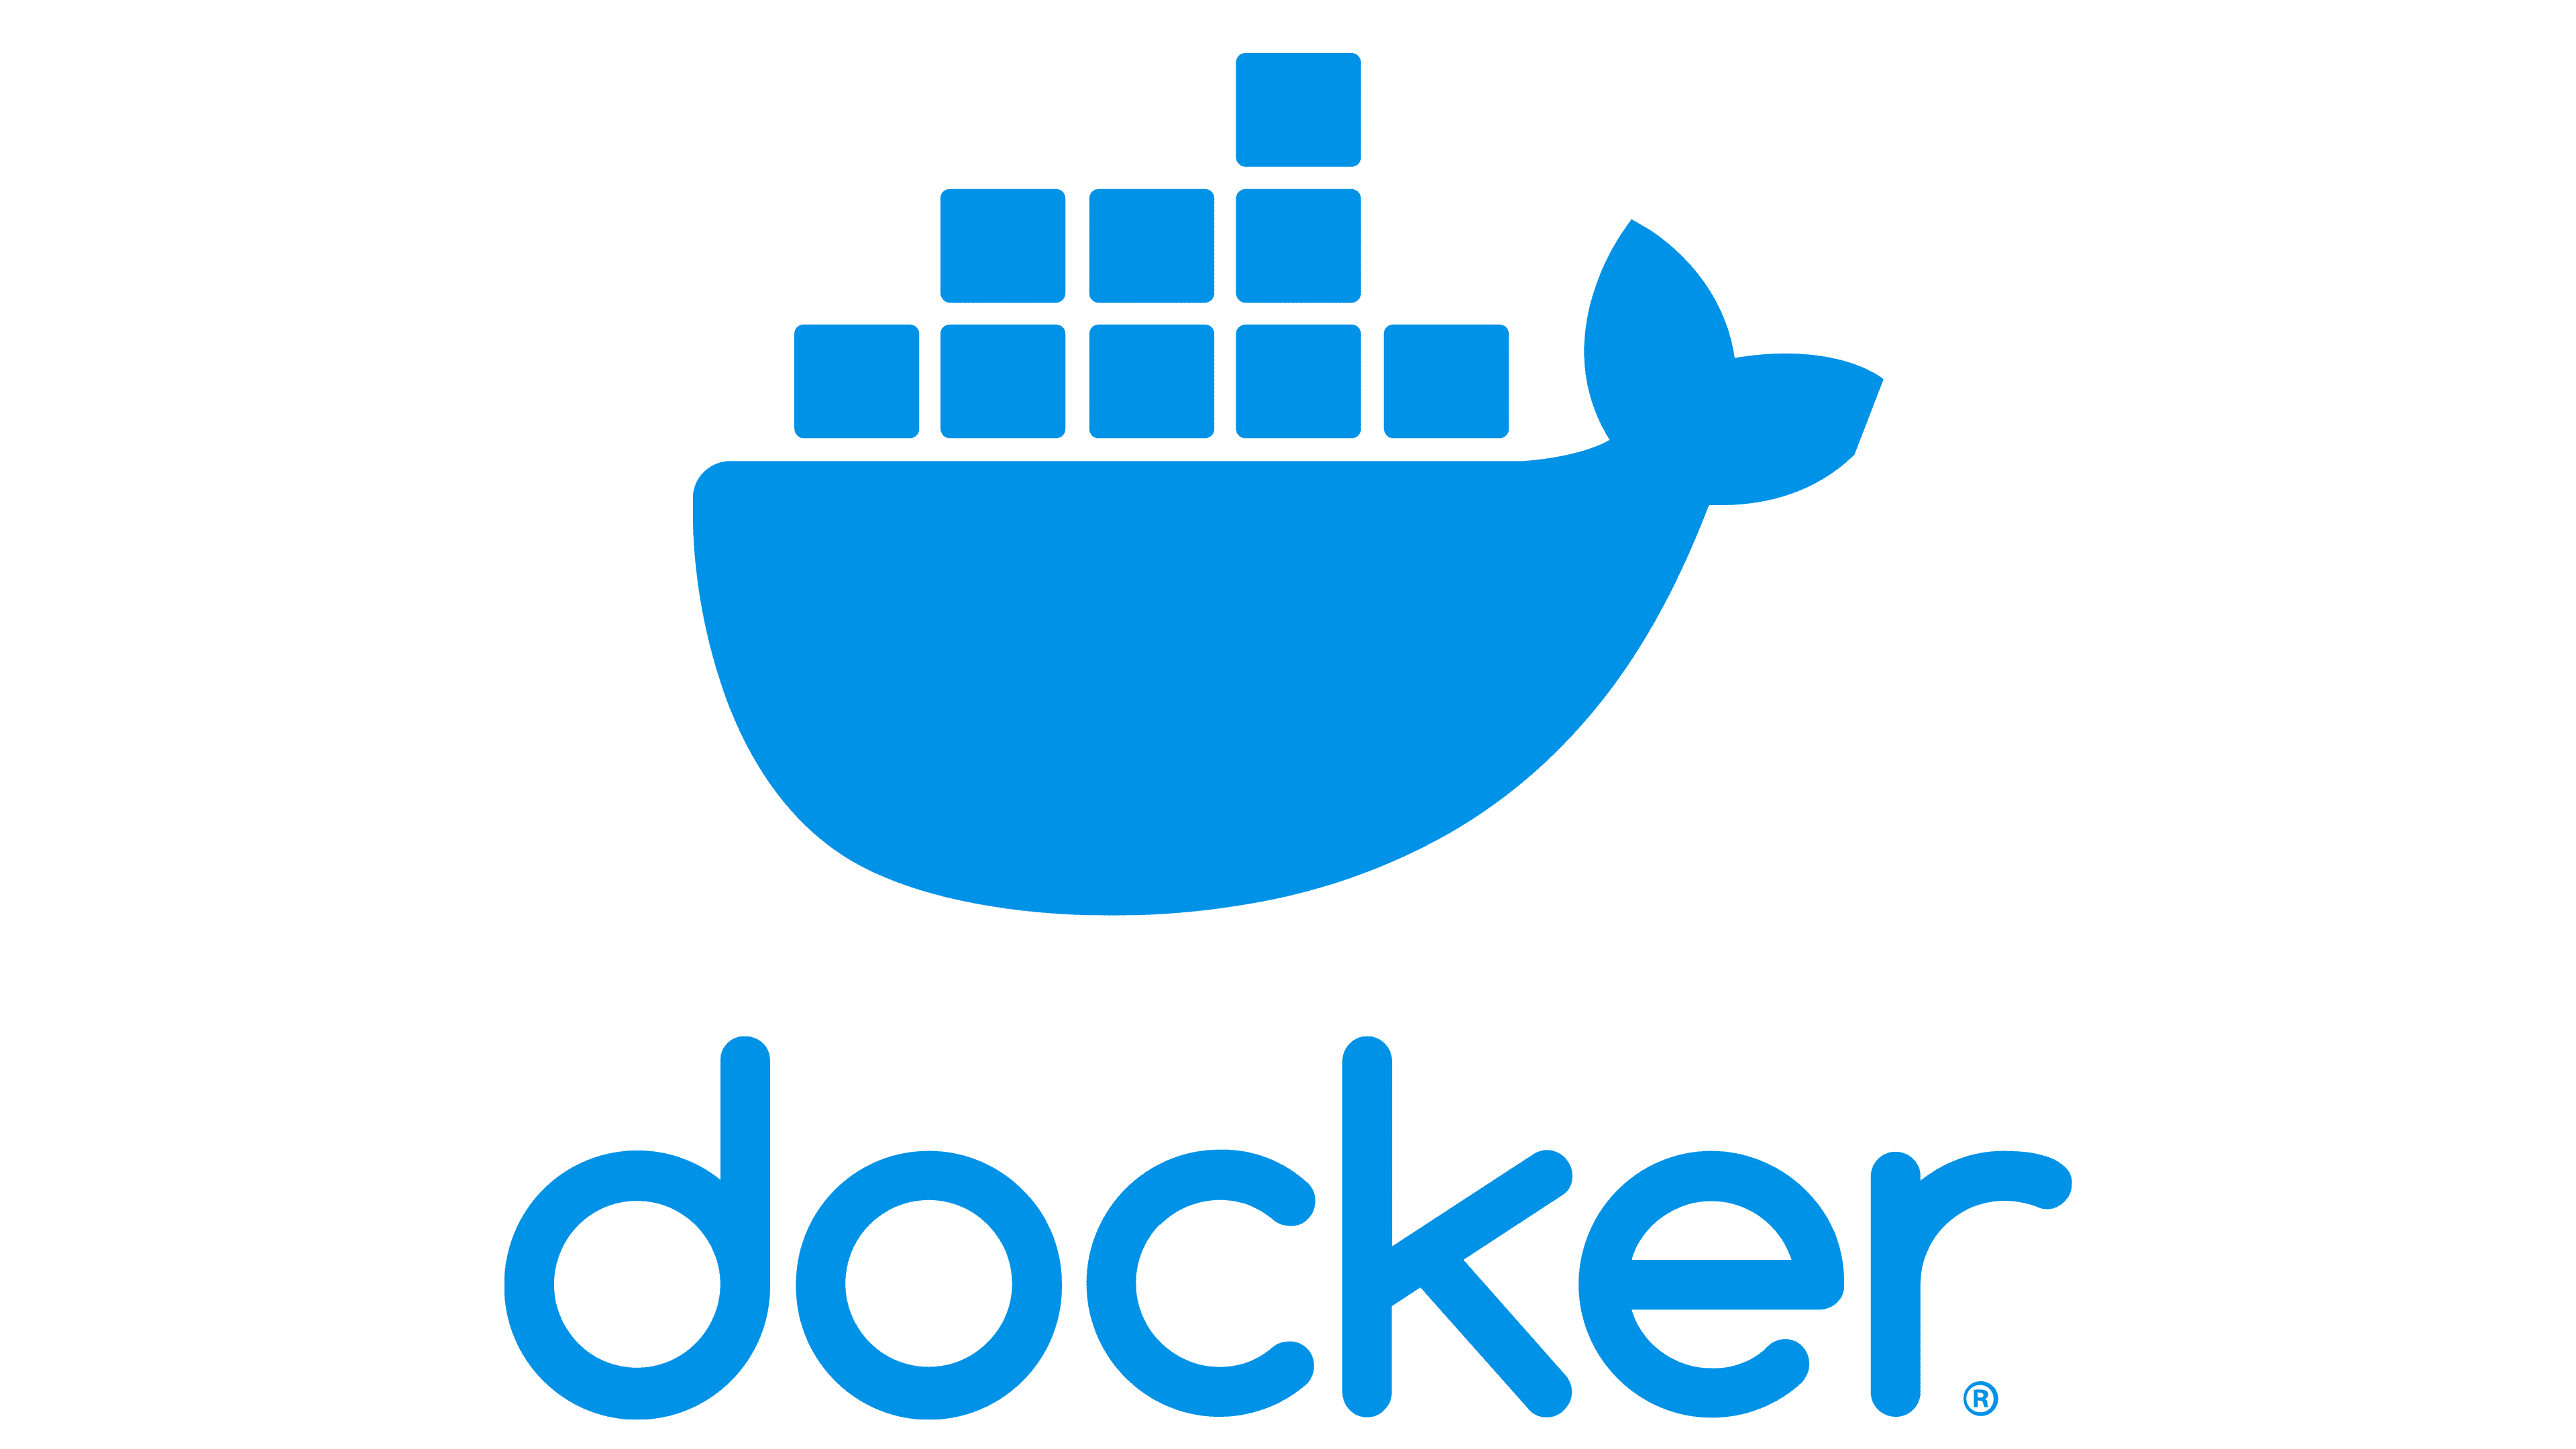
\includegraphics[width=3cm]{imagenes/docker.png}
	\caption{Logo de Docker}
	\label{fig:docker}
\end{figure}

Docker es una plataforma de contenerización que permite empaquetar aplicaciones y sus dependencias en contenedores ligeros y portables, garantizando que se ejecuten de la misma forma en cualquier entorno.

Características principales:
\begin{itemize}
	\item Aislamiento de la aplicación y sus dependencias en contenedores.
	\item Portabilidad: el mismo contenedor funciona en desarrollo, pruebas y producción.
	\item Definición de la infraestructura como código mediante \texttt{Dockerfile} y \texttt{docker-compose.yml}.
	\item Compatibilidad de despliegue en la mayoría de servidores o servicios en la nube.
	\item Reducción de conflictos entre entornos de desarrollo y producción.
\end{itemize}

\subsubsection{Git y GitHub}

\begin{figure}[htb]
	\centering
	\begin{minipage}{0.45\textwidth}
		\centering
		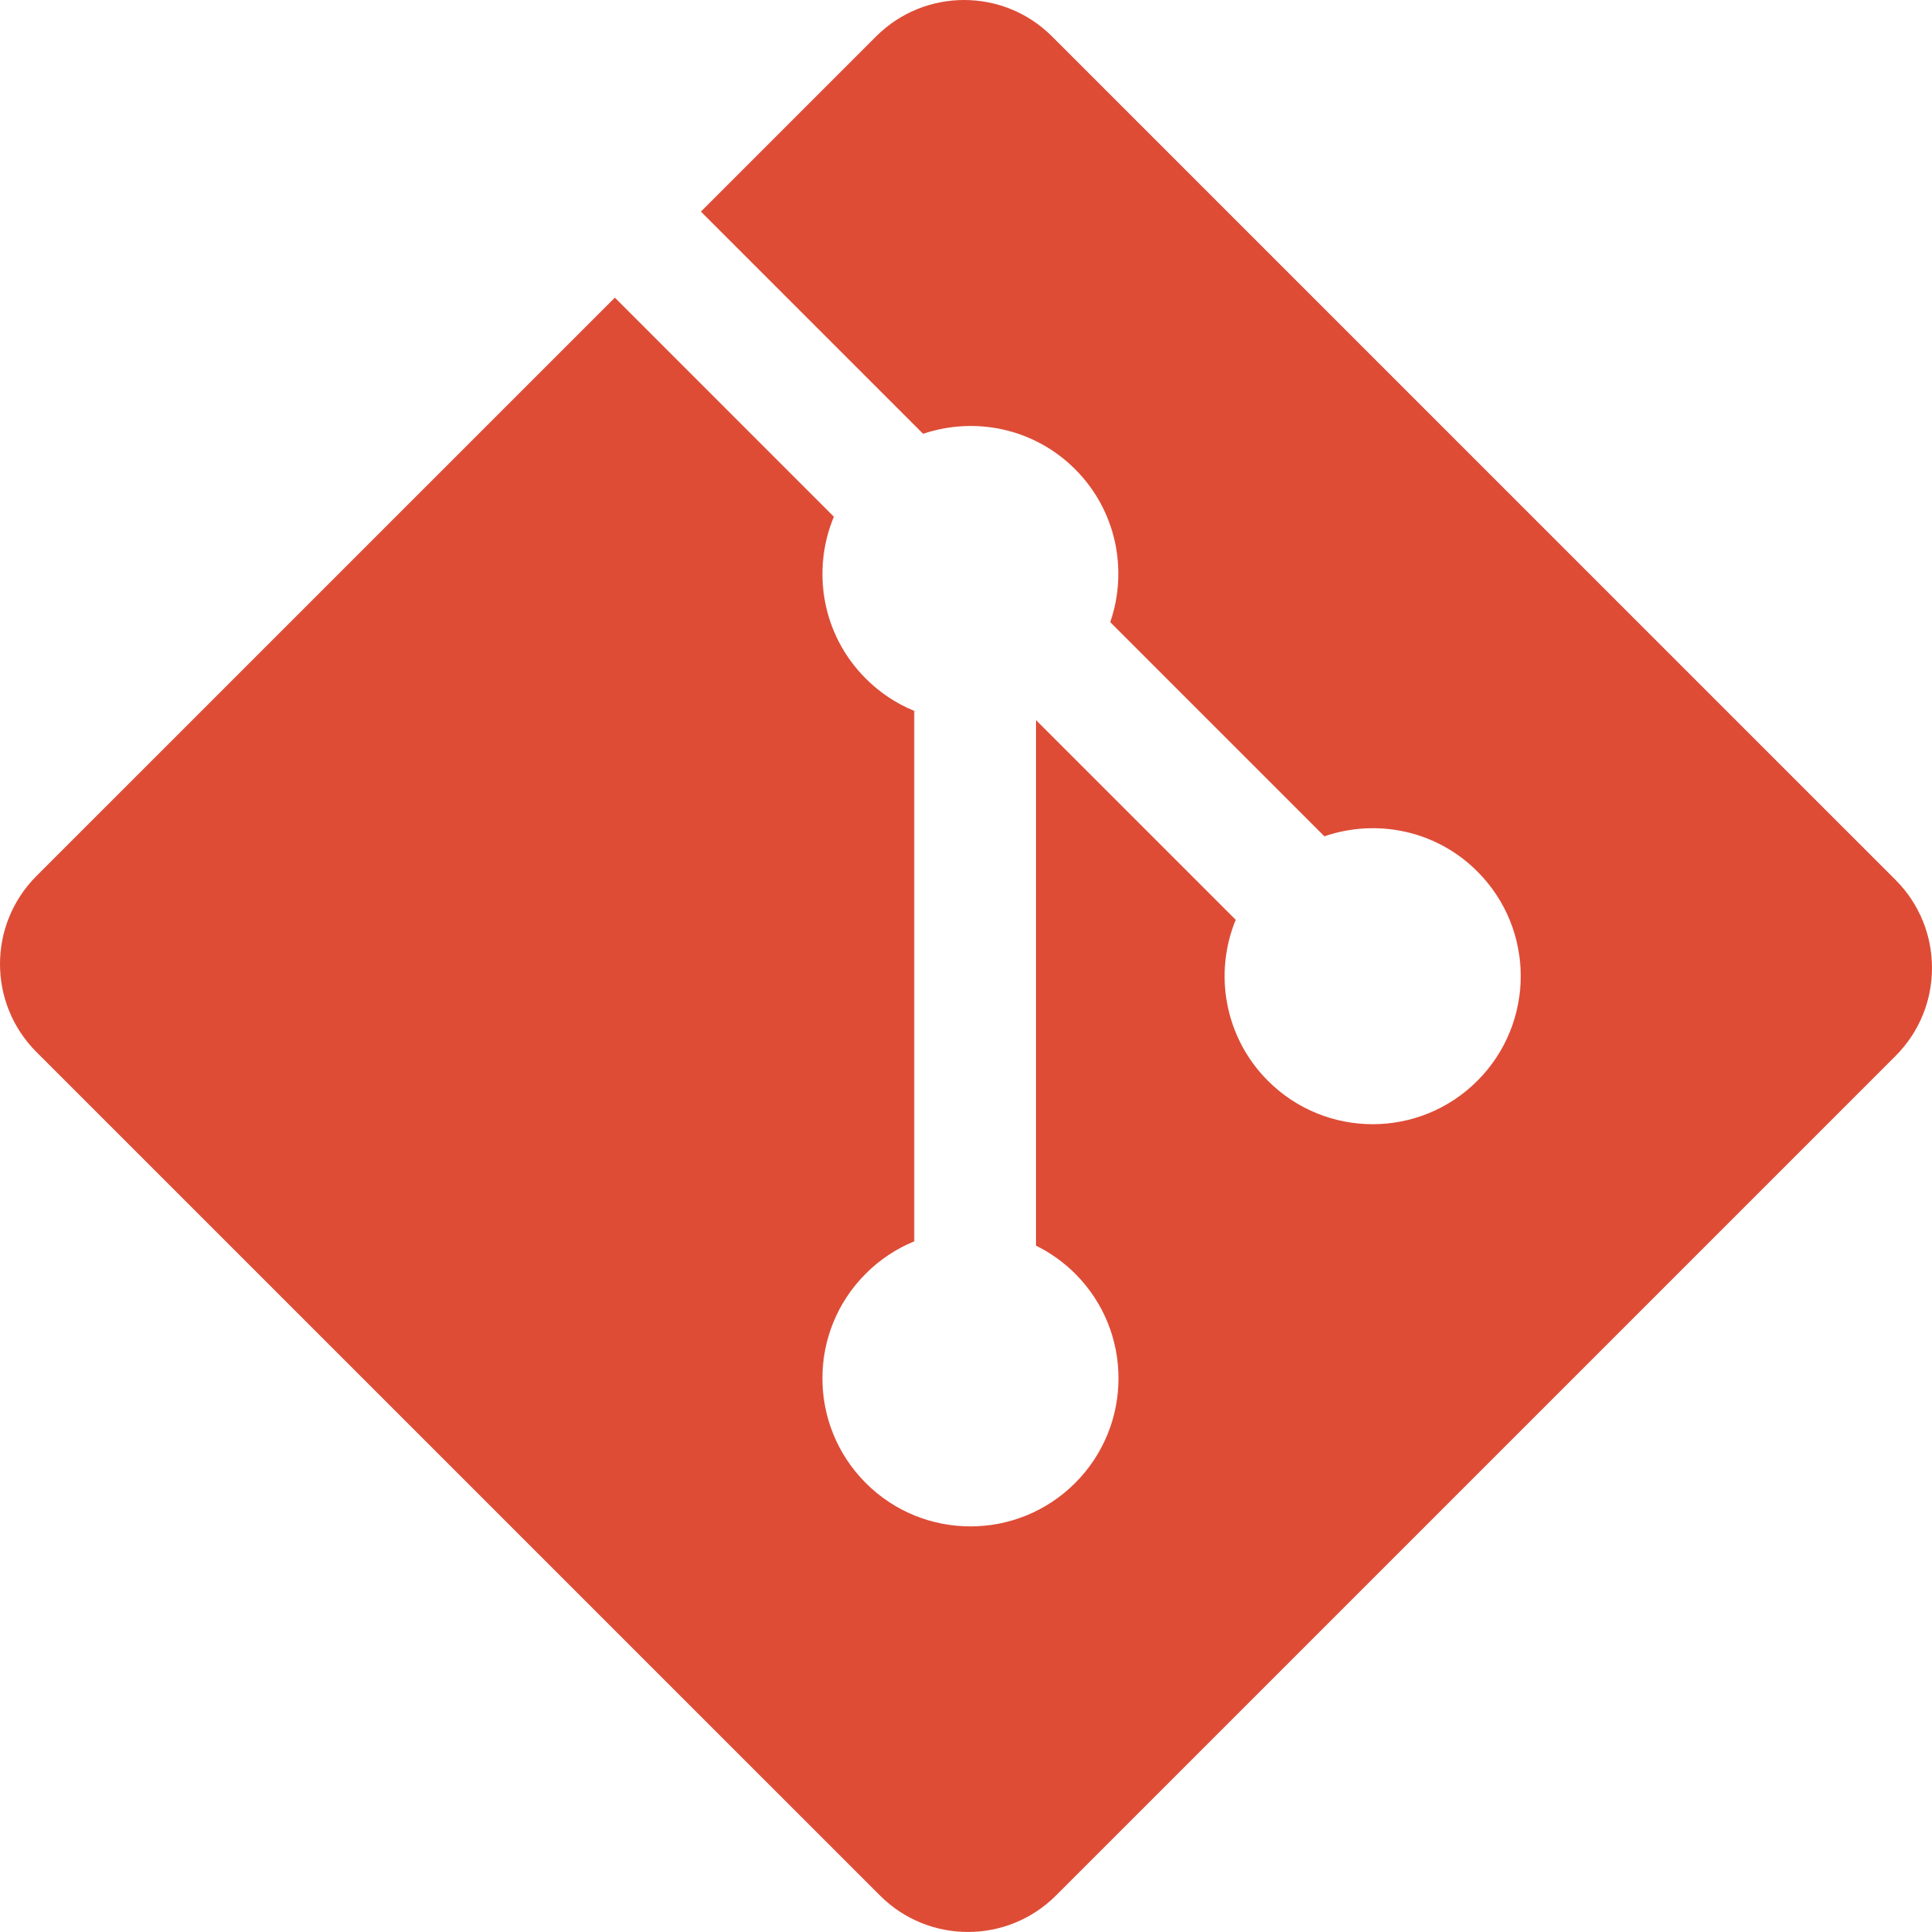
\includegraphics[width=3cm]{imagenes/git.png}
		\caption{Logo de Git}
		\label{fig:git}
	\end{minipage}
	\hfill
	\begin{minipage}{0.45\textwidth}
		\centering
		
\includegraphics[width=3cm]{imagenes/github.png}
		\caption{Logo de GitHub}
		\label{fig:github}
	\end{minipage}
\end{figure}

Git es un sistema de control de versiones distribuido que permite registrar los cambios en el código y colaborar con otros desarrolladores. GitHub es una plataforma basada en Git que permite alojar y gestionar repositorios de código de forma remota y colaborativa.

Características principales:
\begin{itemize}
	\item Control de versiones distribuido que evita pérdidas de código y permite revertir cambios.
	\item Trabajo con ramas para desarrollar funcionalidades de forma segura sin afectar a la versión principal.
	\item Fusión de ramas (\textit{merge}) y resolución de conflictos.
	\item Gestión de \textit{issues} y \textit{pull requests} en GitHub.
	\item Histórico completo de cambios y aportaciones.
	\item Integración con CI/CD para automatización de pruebas y despliegues.
\end{itemize}

\subsubsection{pgAdmin}
\begin{figure}[htb]
	\centering
	
\includegraphics[width=3cm]{imagenes/pgadmin.png}
	\caption{Logo de pgAdmin}
	\label{fig:pgadmin}
\end{figure}

pgAdmin es una herramienta gráfica de administración para PostgreSQL que permite gestionar bases de datos, ejecutar consultas y visualizar datos sin necesidad de utilizar la línea de comandos.

Características principales:
\begin{itemize}
	\item Interfaz visual intuitiva para la gestión de bases de datos.
	\item Editor SQL con resaltado de sintaxis y autocompletado.
	\item Visualización de datos en tablas y exportación en varios formatos.
	\item Gestión de usuarios, roles y permisos.
	\item Monitorización del rendimiento y de las consultas ejecutadas.
\end{itemize}

\subsection{Documentación}

\subsubsection{LaTeX}
\begin{figure}[htb]
	\centering
	
\includegraphics[width=3cm]{imagenes/latex.png}
	\caption{Logo de LaTeX}
	\label{fig:latex}
\end{figure}

LaTeX es un sistema de composición de documentos de alta calidad, ampliamente utilizado en el ámbito académico y científico para la redacción de tesis, artículos y memorias.

Características principales:
\begin{itemize}
	\item Composición tipográfica profesional y consistente.
	\item Gestión automática de índices, referencias cruzadas y bibliografía.
	\item Separación entre contenido y formato, lo que facilita el mantenimiento del documento.
	\item Amplia variedad de paquetes para tablas, figuras, código fuente y matemáticas.
	\item Ideal para documentos extensos como memorias de TFG.
\end{itemize}

\subsubsection{TeXstudio}
\begin{figure}[htb]
	\centering
	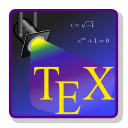
\includegraphics[width=3cm]{imagenes/texstudio.png}
	\caption{Logo de TeXstudio}
	\label{fig:texstudio}
\end{figure}

TeXstudio es un editor de código abierto específicamente diseñado para trabajar con LaTeX. Proporciona un entorno integrado que facilita la escritura, compilación y visualización de documentos LaTeX, con funcionalidades pensadas para agilizar el trabajo con documentos extensos.

Características principales:
\begin{itemize}
	\item Editor con resaltado de sintaxis específico para LaTeX.
	\item Autocompletado de comandos, entornos y referencias bibliográficas.
	\item Visor de PDF integrado con sincronización entre el código fuente y el documento compilado.
	\item Gestión de la estructura del documento mediante un árbol de secciones, figuras, tablas y etiquetas.
	\item Configuración de la cadena de compilación (PdfLaTeX, Biber, etc.) y detección automática de errores.
	\item Integración con Git y otros sistemas de control de versiones.
\end{itemize}

\subsubsection{draw.io}
\begin{figure}[htb]
	\centering
	
\includegraphics[width=3cm]{imagenes/drawio.png}
	\caption{Logo de draw.io}
	\label{fig:drawio}
\end{figure}

draw.io es una herramienta de diagramación de código abierto que permite crear diagramas de flujo, diagramas entidad-relación, diagramas UML y esquemas de arquitectura de software de forma visual e intuitiva.

Características principales:
\begin{itemize}
	\item Interfaz gráfica basada en arrastrar y soltar, sin necesidad de escribir código.
	\item Amplia biblioteca de formas y plantillas para diagramas UML, ER, redes, arquitecturas, etc.
	\item Exportación en múltiples formatos (PNG, SVG, PDF, XML) y opciones de incrustación en documentos.
	\item Integración con Google Drive, OneDrive, GitHub y otras plataformas de almacenamiento.
	\item Funciona tanto en la versión web como en la versión de escritorio, sin necesidad de conexión a Internet en esta última.
	\item Código abierto y gratuito, sin restricciones de uso ni marcas de agua.
\end{itemize}

En el contexto de este proyecto, draw.io se ha utilizado para elaborar los diagramas de arquitectura del sistema, los modelos entidad-relación de la base de datos y los diagramas de flujo de los principales procesos de la aplicación, facilitando la comprensión visual del diseño antes de su implementación.